\documentclass[12pt]{book} % Change to book
\usepackage{amsmath} % for mathematical expressions
\usepackage{xcolor} % for colored text
\usepackage{graphicx} % for including images
\usepackage{url}
\usepackage{booktabs} % for better-looking tables
\usepackage{makecell}
\usepackage{indentfirst}
\usepackage{algorithm}
\usepackage{algpseudocode}
\usepackage{amssymb}
\usepackage{placeins} % For \FloatBarrier
\usepackage{listings}
% Define the language style for Python code
\lstset{
    language=Python,
    basicstyle=\ttfamily,
    keywordstyle=\color{blue},
    stringstyle=\color{red},
    commentstyle=\color{gray},
    morecomment=[l][\color{magenta}]{\#},
    frame=single,
    breaklines=true
}
\begin{document}
\chapter{Dynamic Programming and Network Flow}
\section{Introduction to Dynamic Programming and Network Flow}

\subsection{Overview and Definitions}
Dynamic Programming (DP) and Network Flow are two fundamental concepts in computer science and optimization. 

\textbf{Dynamic Programming} is a method for solving complex problems by breaking them down into simpler subproblems and solving each subproblem only once, storing the solution to each subproblem to avoid redundant computations. It's typically used for optimization problems where the solution can be represented as a sequence of decisions.

\textbf{Network Flow} refers to the study of flows in networks, such as transportation networks, computer networks, and flow networks. The most common problem in network flow is the \textit{maximum flow} problem, where the goal is to find the maximum amount of flow that can be sent from a source node to a sink node in a flow network.

\subsection{Historical Context and Development}
The concept of Dynamic Programming was first introduced by Richard Bellman in the 1950s. He used it to solve optimization problems in operations research and control theory. One of the earliest applications of DP was the \textit{Bellman Equation}, which is fundamental in the field of reinforcement learning.

Network Flow algorithms have a rich history dating back to the mid-20th century. The \textit{max-flow min-cut theorem}, proved by Ford and Fulkerson in 1956, laid the theoretical foundation for many network flow algorithms. Since then, various algorithms such as Ford-Fulkerson, Edmonds-Karp, and Push-Relabel have been developed to efficiently solve network flow problems.

\subsection{Importance in Computational Problems}
Dynamic Programming and Network Flow are indispensable tools in solving a wide range of computational problems.

\textbf{Dynamic Programming} is crucial in solving problems that exhibit the \textit{optimal substructure} property, where the optimal solution to the problem can be constructed from optimal solutions to its subproblems. It's commonly used in various domains such as algorithm design, artificial intelligence, economics, and bioinformatics.

\textbf{Network Flow} algorithms are essential in optimizing the flow of resources in various real-world systems. They have applications in transportation planning, network routing, resource allocation, and computer network design. For example, in transportation, network flow algorithms can be used to optimize traffic flow, minimize congestion, and maximize the efficiency of transportation networks.


\section{Fundamentals of Dynamic Programming}

\subsection{Core Principles of Dynamic Programming}
Dynamic Programming (DP) relies on two core principles:

\begin{enumerate}
    \item \textbf{Optimal Substructure:} The optimal solution to a problem can be constructed from optimal solutions to its subproblems.
    \item \textbf{Overlapping Subproblems:} The problem can be broken down into smaller subproblems, and the same subproblems occur multiple times in the computation.
\end{enumerate}

By exploiting these principles, DP algorithms can efficiently solve optimization problems by avoiding redundant computations.

\subsection{Problem Solving with Dynamic Programming}
Dynamic Programming can be applied to solve a wide range of problems, including:
\begin{itemize}
    \item Shortest path problems
    \item Knapsack problems
    \item Sequence alignment problems
    \item Cutting stock problems
    \item Resource allocation problems
\end{itemize}

The key steps in solving a problem using DP are:
\begin{enumerate}
    \item \textbf{Identify optimal substructure:} Determine how the problem can be divided into smaller subproblems.
    \item \textbf{Formulate recurrence relation:} Express the solution to each subproblem in terms of solutions to its smaller subproblems.
    \item \textbf{Memoization or tabulation:} Store the solutions to subproblems to avoid redundant computations.
\end{enumerate}

\subsection{Applications and Examples}
Dynamic Programming finds applications in various domains due to its ability to efficiently solve optimization problems. Some notable applications include:

\begin{itemize}
    \item \textbf{Shortest Path Problems:} Dynamic Programming can be used to find the shortest path in a graph from a source node to a destination node. The classic example is Dijkstra's algorithm, which efficiently finds the shortest path in a weighted graph.
    
    \item \textbf{Knapsack Problems:} Dynamic Programming can solve the knapsack problem efficiently. Given a set of items, each with a weight and a value, determine the maximum value that can be obtained by selecting a subset of items that fit into a knapsack of a given capacity.
    
    \item \textbf{Sequence Alignment:} In bioinformatics, Dynamic Programming is used to align sequences of DNA, RNA, or proteins. The Needleman-Wunsch algorithm, for example, performs global sequence alignment to find the best match between two sequences.
    
    \item \textbf{Cutting Stock Problems:} Dynamic Programming can be applied to cutting stock problems, where the goal is to cut raw materials into smaller pieces to meet specific demands while minimizing waste. This has applications in manufacturing and production planning.
    
    \item \textbf{Resource Allocation Problems:} Dynamic Programming is used in resource allocation problems, such as scheduling tasks to minimize time or cost. For example, the classic job scheduling problem can be efficiently solved using Dynamic Programming techniques.
\end{itemize}

These are just a few examples of the diverse range of problems that can be tackled using Dynamic Programming. Its versatility and efficiency make it a powerful tool in algorithm design and optimization.

\textbf{Algorithmic Example}

Let's consider the classic example of solving the Fibonacci sequence using dynamic programming. The Fibonacci sequence is defined as:
\[ F(n) = F(n-1) + F(n-2) \]
with base cases \( F(0) = 0 \) and \( F(1) = 1 \).

We can solve this problem efficiently using dynamic programming by storing the solutions to subproblems:
\FloatBarrier
\begin{algorithm}
\caption{Dynamic Programming for Fibonacci Sequence}\label{fib_dp}
\begin{algorithmic}[1]
\Procedure{Fibonacci}{$n$}
\State $F[0] \gets 0$
\State $F[1] \gets 1$
\For{$i \gets 2$ to $n$}
\State $F[i] \gets F[i-1] + F[i-2]$
\EndFor
\State \textbf{return} $F[n]$
\EndProcedure
\end{algorithmic}
\end{algorithm}
\FloatBarrier
\textbf{Python Implementation}

Here's a Python implementation of the Fibonacci sequence using dynamic programming:
\FloatBarrier
\begin{lstlisting}
def fibonacci(n):
    F = [0] * (n + 1)
    F[0] = 0
    F[1] = 1
    for i in range(2, n + 1):
        F[i] = F[i - 1] + F[i - 2]
    return F[n]
\end{lstlisting}
\FloatBarrier
This implementation has a time complexity of \( O(n) \) and space complexity of \( O(n) \), making it efficient for computing large Fibonacci numbers.


\section{Introduction to Network Flow}

\subsection{Basic Concepts and Terminologies}
Network Flow refers to the study of flows in networks, where a network consists of nodes and edges. 

\textbf{Nodes} represent entities such as sources, sinks, or intermediate points in the network.

\textbf{Edges} represent connections between nodes and are associated with capacities, indicating the maximum amount of flow that can pass through them.

\textbf{Flow} refers to the amount of some commodity (such as goods, data, or traffic) passing through the edges of the network.

\textbf{Source} is a node where the flow originates, and \textbf{sink} is a node where the flow terminates.

\subsection{Applications of Network Flow}
Network Flow problems have numerous applications across various domains:

\begin{itemize}
    \item \textbf{Transportation Planning:} Optimizing traffic flow in road networks, scheduling transportation routes, and minimizing congestion.
    \item \textbf{Telecommunications:} Routing data packets through computer networks efficiently.
    \item \textbf{Supply Chain Management:} Optimizing the flow of goods through supply chains, minimizing transportation costs, and maximizing efficiency.
    \item \textbf{Energy Networks:} Maximizing the flow of electricity through power grids, minimizing transmission losses.
    \item \textbf{Water Networks:} Managing water distribution in irrigation systems, ensuring equitable distribution of water resources.
\end{itemize}

\subsection{Problem Formulation and Examples}
The fundamental problem in Network Flow is to determine the maximum amount of flow that can be sent from a source node to a sink node in a flow network, subject to capacity constraints on edges.

Given a directed graph \( G = (V, E) \), where \( V \) is the set of nodes and \( E \) is the set of edges, along with a source node \( s \) and a sink node \( t \), the goal is to find the maximum flow \( f \) from \( s \) to \( t \) while satisfying the capacity constraints on the edges.

\subsubsection{Algorithmic Example}
Consider the following network:

\begin{center}
\begin{tabular}{ c c c }
    \textbf{Node 1} & \textbf{Node 2} & \textbf{Node 3} \\
    \hline
    $s$ & & $t$ \\
    & 5 & \\
    3 & 2 & \\
    & 4 & \\
\end{tabular}
\end{center}

The numbers on the edges represent their capacities. Using the Ford-Fulkerson algorithm, we can find the maximum flow from \( s \) to \( t \) in this network.

\subsubsection{Python Code}
Here's an example of a Python implementation of the Ford-Fulkerson algorithm:

\begin{lstlisting}
def ford_fulkerson(graph, source, sink):
    max_flow = 0
    residual_graph = graph
    
    while True:
        # Use BFS to find an augmenting path
        path = bfs(residual_graph, source, sink)
        
        if not path:
            break
        
        # Find the minimum capacity in the augmenting path
        min_capacity = min(residual_graph[u][v] for u, v in zip(path, path[1:]))
        
        # Update residual capacities along the augmenting path
        for u, v in zip(path, path[1:]):
            residual_graph[u][v] -= min_capacity
            residual_graph[v][u] += min_capacity
        
        # Add the flow of the augmenting path to the max flow
        max_flow += min_capacity
    
    return max_flow
\end{lstlisting}
\FloatBarrier
This code implements the Ford-Fulkerson algorithm to find the maximum flow in a flow network represented by a graph.

\textbf{Examples of Network Flow}
\textbf{Example 1: Transportation Network}
Consider a transportation network with cities represented as nodes and roads represented as edges. The capacities of the edges represent the maximum number of vehicles that can travel on each road. The goal is to maximize the flow of vehicles from a source city to a destination city while avoiding congestion.

\textbf{Example 2: Telecommunications Network}
In a telecommunications network, nodes represent switching stations, and edges represent communication links. The capacities of the edges represent the maximum bandwidth of each link. The objective is to route data packets from a source node to a destination node while minimizing delays and maximizing network throughput.

\textbf{Example 3: Supply Chain Management}
Consider a supply chain network with warehouses as nodes and transportation routes as edges. The capacities of the edges represent the maximum quantity of goods that can be transported along each route. The goal is to optimize the flow of goods from suppliers to customers, minimizing transportation costs and maximizing efficiency.

\textbf{Example 4: Energy Distribution Network}
In an energy distribution network, nodes represent power stations, substations, and consumers, while edges represent transmission lines. The capacities of the edges represent the maximum amount of electricity that can be transmitted along each line. The objective is to maximize the flow of electricity from power stations to consumers while minimizing transmission losses and ensuring grid stability.

\textbf{Example 5: Water Distribution Network}
In a water distribution network, nodes represent reservoirs, treatment plants, and distribution points, while edges represent pipelines. The capacities of the edges represent the maximum flow rate of water through each pipeline. The goal is to optimize the distribution of water resources, ensuring equitable access to clean water and minimizing leakage.

These examples illustrate the diverse applications of Network Flow in various real-world scenarios, highlighting its importance in optimizing the flow of resources in complex networks.


\section{Maximum Flow Theory}

\subsection{Understanding Maximum Flow Problems}
In network flow theory, the \textbf{maximum flow problem} is a fundamental optimization problem that seeks to determine the maximum amount of flow that can be sent from a source node to a sink node in a flow network. Each edge in the network has a capacity that represents the maximum amount of flow it can carry. The goal is to find a flow assignment that maximizes the total flow from the source to the sink while satisfying the capacity constraints and flow conservation at intermediate nodes.

\subsection{The Ford-Fulkerson Algorithm}
The Ford-Fulkerson algorithm is a classical method for solving the maximum flow problem. It operates by iteratively finding augmenting paths from the source to the sink and updating the flow along these paths until no more augmenting paths exist. The algorithm's core idea is to increase the flow along augmenting paths until no more paths can be found, resulting in the maximum flow.

\subsubsection{Algorithm Description}
The Ford-Fulkerson algorithm is a classic method for solving the maximum flow problem in a flow network. It operates by iteratively finding augmenting paths from the source to the sink and updating the flow along these paths until no more augmenting paths exist.

At each iteration of the algorithm, we start with an initial feasible flow assignment, often initialized to zero. Then, we use a technique such as depth-first search (DFS) or breadth-first search (BFS) to find an augmenting path from the source to the sink in the residual graph. An augmenting path is a simple path from the source to the sink such that all edges along the path have residual capacity greater than zero.

Once we find an augmenting path, we determine the maximum amount of flow that can be sent along this path without violating any capacity constraints. This value is called the residual capacity of the augmenting path. We then update the flow along the path by adding this residual capacity to the flow values of the edges in the path.

This process repeats until no more augmenting paths can be found in the residual graph. At this point, the flow assignment obtained is a maximum flow, as there are no more paths from the source to the sink with residual capacity.


\subsubsection{Implementation Details}
Implementing the Ford-Fulkerson algorithm requires maintaining a residual graph, which represents the remaining capacity on each edge after the flow has been assigned. Additionally, one needs to use a suitable path-finding algorithm to efficiently find augmenting paths, such as DFS or BFS.

The implementation of the Ford-Fulkerson algorithm involves maintaining a residual graph, which represents the remaining capacity on each edge after the flow has been assigned. Additionally, a suitable path-finding algorithm such as depth-first search (DFS) or breadth-first search (BFS) is used to efficiently find augmenting paths.
\FloatBarrier
\begin{figure}[h]
    \centering
    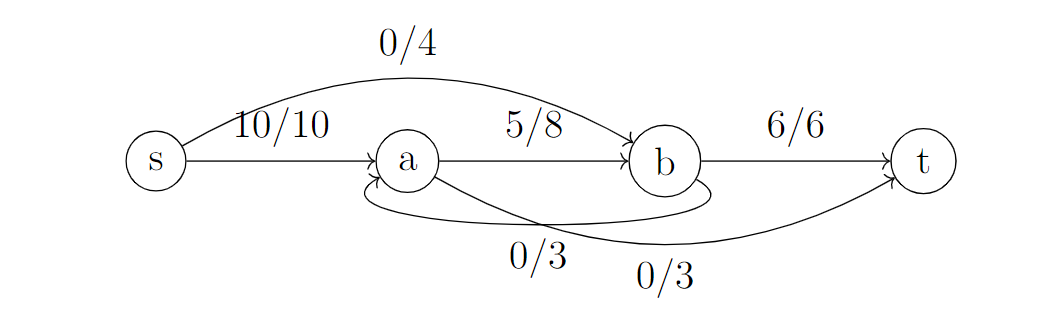
\includegraphics[width=0.6\textwidth]{images/Visualization_of_Ford_Fulkerson_Algorithm.png}
    \caption{Visualization of the Ford-Fulkerson Algorithm}
\end{figure}
\FloatBarrier
\textbf{Python Implementation}

Here's a simple Python implementation of the Ford-Fulkerson algorithm:
\FloatBarrier
\begin{lstlisting}
# Pseudocode for Ford-Fulkerson Algorithm
def ford_fulkerson(graph, source, sink):
    residual_graph = initialize_residual_graph(graph)
    max_flow = 0
    while True:
        path = find_augmenting_path(residual_graph, source, sink)
        if not path:
            break
        augment(residual_graph, path)
        max_flow += path_flow
    return max_flow
\end{lstlisting}
\FloatBarrier
\subsubsection{Applications and Limitations of Maximum Flow Problems}
Maximum flow problems have numerous applications across various domains, including transportation, network design, and resource allocation. They can be used to model scenarios such as traffic flow optimization, network routing, and capacity planning.

However, the Ford-Fulkerson algorithm may not always terminate or produce correct results if the capacities have fractional values or if there are negative capacity cycles in the graph. Additionally, its time complexity can be high in certain cases, leading to inefficient performance on large graphs.

\subsection{The Push-Relabel Algorithm}
The Push-Relabel algorithm is another approach to solving the maximum flow problem, known for its efficiency and simplicity.

\subsubsection{Algorithm Overview}
The Push-Relabel algorithm is an alternative approach to solving the maximum flow problem, known for its efficiency and simplicity. Unlike the Ford-Fulkerson algorithm, which iteratively searches for augmenting paths, the Push-Relabel algorithm operates by maintaining a preflow and performing local operations to gradually transform it into a maximum flow.

The key idea behind the Push-Relabel algorithm is to push excess flow from nodes with surplus to nodes with deficits while maintaining certain properties to ensure convergence to the maximum flow. This is achieved through two main operations: pushing and relabeling.

\textbf{Push operation:} If a node \(u\) has excess flow (i.e., the flow into \(u\) exceeds the flow out of \(u\)), we push this excess flow along the outgoing edges to neighboring nodes with deficits. This operation helps redistribute the flow in the network and reduce excess at certain nodes.

\textbf{Relabel operation:} If a node \(u\) has excess flow but cannot push it along any outgoing edge due to capacity constraints, we relabel \(u\) by increasing its label (height) to create a path for the excess flow to move out of \(u\) in future iterations. This operation ensures progress towards the maximum flow while maintaining feasibility.

The Push-Relabel algorithm repeats these operations until all nodes reach a state of balance, where the flow into each node equals the flow out of it. At this point, the preflow becomes a maximum flow, and the algorithm terminates.

The Push-Relabel algorithm maintains a preflow, which is a feasible but not necessarily maximum flow. It iteratively pushes excess flow from nodes with surplus to nodes with deficits while maintaining certain properties to ensure convergence to the maximum flow.
\FloatBarrier
\begin{figure}[h]
    \centering
    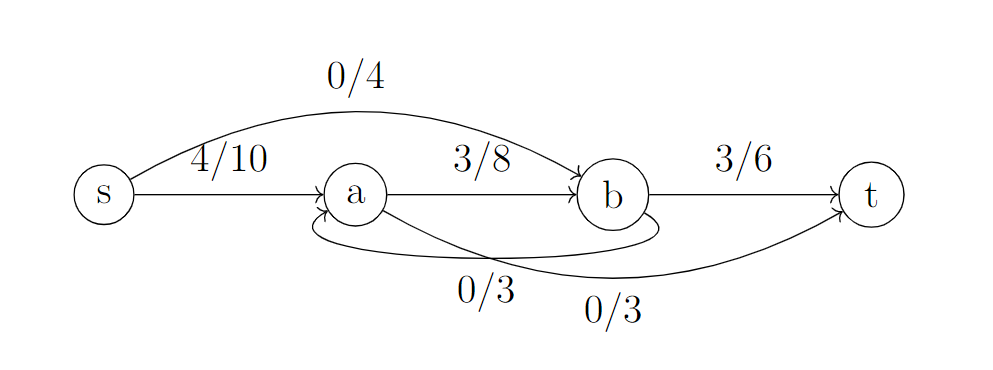
\includegraphics[width=0.6\textwidth]{images/Visualization_of_Push_Relabel_Algorithm.png}
    \caption{Visualization of the Push-Relabel Algorithm}
\end{figure}
\FloatBarrier
In the graphical representations above, the nodes represent vertices in the flow network, and the edges represent the flow between vertices. The capacities of the edges are indicated by the thickness or color intensity of the edges. During the execution of the algorithms, the flow along the edges is updated iteratively until a maximum flow is achieved.

\textbf{Python Implementation}
Here's a basic Python implementation of the Push-Relabel algorithm:
\FloatBarrier
\begin{lstlisting}
# Pseudocode for Push-Relabel Algorithm
def push_relabel(graph, source, sink):
    initialize_preflow(graph, source)
    while excess_nodes_exist(graph):
        u = find_node_with_excess(graph)
        if not discharge(u):
            relabel(u)
    return compute_max_flow(graph)
\end{lstlisting}

\subsubsection{Efficiency and Performance}
The efficiency and performance of the Push-Relabel algorithm can be analyzed in terms of its time complexity and its behavior on different types of graphs.

The time complexity of the Push-Relabel algorithm is typically analyzed using the concept of \textit{work} and \textit{depth}. The \textit{work} represents the total number of operations performed by the algorithm, while the \textit{depth} measures the maximum number of operations required to push excess flow from a node to the sink. In practice, the time complexity of the Push-Relabel algorithm is often expressed as \(O(V^2 \sqrt{E})\), where \(V\) is the number of vertices and \(E\) is the number of edges in the graph.

To understand the time complexity intuitively, consider that the algorithm performs a sequence of \textit{push} and \textit{relabel} operations. Each \textit{push} operation takes \(O(1)\) time, while each \textit{relabel} operation takes \(O(V)\) time in the worst case. The number of \textit{push} operations required to reach the maximum flow is bounded by \(O(V^2)\), and the number of \textit{relabel} operations is bounded by \(O(VE)\) in the worst case. Therefore, the overall time complexity is \(O(V^2 \sqrt{E})\).

The Push-Relabel algorithm tends to perform well on dense graphs, where the number of edges is proportional to the square of the number of vertices. In such graphs, the algorithm's time complexity is closer to its best-case scenario. However, on sparse graphs, where the number of edges is much smaller than the square of the number of vertices, the algorithm's performance may degrade, approaching its worst-case time complexity.


\subsubsection{Comparison with Ford-Fulkerson}
When comparing the Push-Relabel algorithm with the Ford-Fulkerson algorithm, several factors come into play, including time complexity, implementation complexity, and practical efficiency.

In terms of time complexity, the Ford-Fulkerson algorithm has a worst-case time complexity of \(O(EF)\), where \(E\) is the number of edges and \(F\) is the maximum flow value. In contrast, as mentioned earlier, the Push-Relabel algorithm typically has a worst-case time complexity of \(O(V^2 \sqrt{E})\). Therefore, on dense graphs with a large number of edges, the Push-Relabel algorithm often outperforms Ford-Fulkerson.

From an implementation perspective, the Push-Relabel algorithm may be easier to implement than Ford-Fulkerson, as it does not require explicitly finding augmenting paths. Instead, it maintains a preflow and performs local operations (push and relabel) to reach the maximum flow.

In practice, the choice between the two algorithms depends on the characteristics of the specific problem instance. If the graph is dense or the maximum flow value is large, the Push-Relabel algorithm is likely to be more efficient. However, if the graph is sparse or the maximum flow value is small, Ford-Fulkerson may perform comparably or even better.


\section{Maximum Flow Applications}

\subsection{Assignment Problem}
The assignment problem is a classic optimization problem that involves assigning a set of resources to a set of tasks in a way that minimizes the total cost or maximizes the total profit. Each resource can only be assigned to one task, and each task requires exactly one resource.
\subsubsection{Problem Statement}
Formally, given \(n\) resources and \(n\) tasks, and a cost matrix \(C\) where \(C[i][j]\) represents the cost of assigning resource \(i\) to task \(j\), the goal is to find an assignment that minimizes the total cost or maximizes the total profit.

\subsubsection{Solving with Network Flow}

To solve the assignment problem using network flow, we can model it as a bipartite graph where one set of vertices represents the resources, another set represents the tasks, and the edges represent potential assignments. We then use a maximum flow algorithm to find the optimal assignment.

\textbf{Algorithm:}
\begin{itemize}
    \item Create a bipartite graph with \(n\) vertices representing resources and \(n\) vertices representing tasks.
\item Add a source node \(s\) connected to all resource vertices with edges of capacity 1.
\item Add a sink node \(t\) connected to all task vertices with edges of capacity 1.
\item Set the capacities of the edges connecting resources to tasks according to the cost matrix \(C\).
\item Find the maximum flow from \(s\) to \(t\) using a maximum flow algorithm such as Ford-Fulkerson or Push-Relabel.
\item The maximum flow represents the optimal assignment, and the corresponding flow values determine which resources are assigned to which tasks.
\end{itemize}

\textbf{Python Implementation:}
\FloatBarrier
\begin{lstlisting}
def assignment_problem(cost_matrix):
    n = len(cost_matrix)
    graph = build_graph(cost_matrix)
    max_flow = max_flow_algorithm(graph, source, sink)
    assignments = extract_assignments(max_flow)
    return assignments

def build_graph(cost_matrix):
    # Build bipartite graph with source, sink, and edges
    pass

def max_flow_algorithm(graph, source, sink):
    # Apply maximum flow algorithm
    pass

def extract_assignments(max_flow):
    # Extract assignments from maximum flow
    pass

# Example usage
cost_matrix = [[3, 5, 7], [2, 6, 8], [1, 4, 9]]
assignments = assignment_problem(cost_matrix)
print(assignments)
\end{lstlisting}

\FloatBarrier
\subsubsection{Case Studies and Real-World Applications}

The assignment problem has numerous real-world applications across various domains, including:
\begin{itemize}
    \item  \textbf{Job Scheduling:} Assigning workers to tasks to minimize overall completion time or maximize productivity.
\item \textbf{Transportation Planning:} Assigning vehicles to routes to minimize transportation costs or maximize efficiency.
\item \textbf{Resource Allocation:} Assigning machines to jobs in manufacturing processes to optimize production.
\item \textbf{Project Management:} Assigning team members to project tasks to meet deadlines and budget constraints.
\end{itemize}

These are just a few examples of how the assignment problem can be applied in practice to solve optimization challenges and improve resource utilization.

\section{Advanced Topics in Dynamic Programming}

\subsection{Optimizing Dynamic Programming Solutions}

Dynamic Programming (DP) provides efficient solutions to optimization problems by breaking them down into smaller subproblems. However, as problem size increases, DP solutions can become computationally expensive due to redundant computations. Optimizing DP solutions involves techniques to minimize such redundant computations.

One optimization technique in DP is memoization, which involves storing the results of intermediate subproblems to avoid recomputation. Here's an example of memoization in the context of the Fibonacci sequence:
\FloatBarrier
\begin{algorithm}
initialize an array memo to store Fibonacci numbers
initialize memo[0] to 0 and memo[1] to 1

function fib(n):
    if memo[n] is not defined:
        memo[n] = fib(n-1) + fib(n-2)
    return memo[n]  
\end{algorithm}
\FloatBarrier
\textbf{Explanation:}
\begin{itemize}
    \item The array \texttt{memo} is used to store Fibonacci numbers that have already been calculated.
    \item Initially, \texttt{memo[0]} is set to 0 and \texttt{memo[1]} is set to 1 to handle the base cases of the Fibonacci sequence.
    \item The function \texttt{fib(n)} takes an integer \texttt{n} as input and returns the Fibonacci number corresponding to that index.
    \item If \texttt{memo[n]} is not yet defined, it means that the Fibonacci number for index \texttt{n} has not been calculated yet. In this case, the function recursively calculates \texttt{fib(n-1)} and \texttt{fib(n-2)}, stores the result in \texttt{memo[n]}, and returns it.
    \item If \texttt{memo[n]} is already defined, the function simply returns the precomputed value stored in \texttt{memo[n]}.
\end{itemize}

\textbf{Python Implementation}
\begin{lstlisting}
memo = {}

def fibonacci(n):
    if n in memo:
        return memo[n]
    if n <= 1:
        return n
    memo[n] = fibonacci(n-1) + fibonacci(n-2)
    return memo[n]

# Example usage
print(fibonacci(10))  # Output: 55
\end{lstlisting}
\FloatBarrier
By memoizing the results of intermediate Fibonacci numbers, we avoid redundant computations, leading to significant performance improvements, especially for larger values of \( n \).



\subsection{Dynamic Programming in Distributed Systems}

Dynamic Programming techniques play a crucial role in optimizing resource allocation, scheduling, and load balancing in distributed systems. These systems consist of multiple interconnected nodes or processors, each with its computational capacity and communication capabilities.

In distributed systems, tasks often need to be executed on available resources while considering factors such as resource availability, task dependencies, and communication overhead. Dynamic Programming provides a powerful framework for solving such optimization problems efficiently.


One example of DP in distributed systems is the task scheduling problem, where tasks need to be assigned to available resources to maximize throughput or minimize latency. Here's a simplified example of task scheduling using DP:

The following algorithm performs task scheduling given a list of tasks and available resources:

\begin{algorithm}
\caption{Task Scheduling}\label{task-scheduling}
\begin{algorithmic}[1]
\Procedure{TaskScheduling}{$tasks, resources$}
    \State $dp \gets$ list of zeros of length $(\text{len}(tasks) + 1)$
    \For{$i \gets 1$ \textbf{to} $\text{len}(tasks)$}
        \For{$j \gets \text{len}(resources) - 1$ \textbf{downto} $0$}
            \If{$resources[j] \geq tasks[i-1]$}
                \State $dp[i] \gets \max(dp[i], dp[i-1] + tasks[i-1])$
                \State $resources[j] \gets resources[j] - tasks[i-1]$
            \EndIf
        \EndFor
    \EndFor
    \State \textbf{return} $dp[\text{len}(tasks)]$
\EndProcedure
\end{algorithmic}
\end{algorithm}
\FloatBarrier
\textbf{Explanation:}
\begin{itemize}
    \item The function \texttt{TaskScheduling} takes two input arrays: \texttt{tasks} containing the durations of tasks, and \texttt{resources} containing the available resources.
    \item It initializes an array \texttt{dp} to store the maximum total duration achievable at each task index.
    \item The algorithm iterates over each task and available resource, starting from the last resource. For each task, it checks if the current resource is sufficient to execute the task.
    \item If the resource is sufficient, it updates \texttt{dp[i]} with the maximum total duration achievable by including the current task, and decrements the available resource.
    \item Finally, the algorithm returns the maximum total duration achievable at the last task index, which represents the optimal task scheduling.
\end{itemize}

This algorithm efficiently schedules tasks using dynamic programming and resource constraints.

\textbf{Python Implementation:}
\FloatBarrier
\begin{lstlisting}
def task_scheduling(tasks, resources):
    dp = [0] * (len(tasks) + 1)
    for i in range(1, len(tasks) + 1):
        for j in range(len(resources) - 1, -1, -1):
            if resources[j] >= tasks[i-1]:
                dp[i] = max(dp[i], dp[i-1] + tasks[i-1])
                resources[j] -= tasks[i-1]
    return dp[-1]

# Example usage
tasks = [3, 5, 2, 7]
resources = [10, 8, 6, 12]
print(task_scheduling(tasks, resources))  # Output: 17
\end{lstlisting}
\FloatBarrier
In this example, the DP array `dp[i]` stores the maximum throughput achievable by scheduling the first `i` tasks on the available resources.


\subsection{Recent Advances and Research Directions}

Recent advances in DP have focused on improving scalability, parallelism, and handling of real-time constraints. Additionally, research is exploring the integration of DP techniques with machine learning and deep learning for solving complex optimization problems.


\section{Advanced Network Flow Techniques}

\subsection{Scaling Algorithms for Network Flow}

Scaling algorithms for network flow, such as the Capacity Scaling and the Cost Scaling algorithms, are designed to efficiently solve large-scale network flow problems. These algorithms work by repeatedly augmenting the flow along paths with sufficient residual capacity, scaling up the flow incrementally until the maximum flow is reached.

\textbf{Capacity Scaling Algorithm:}
The Capacity Scaling algorithm works by iteratively scaling up the capacity of the network until it exceeds the maximum flow value. At each iteration, it finds augmenting paths using a scaling factor that gradually increases. This allows the algorithm to focus on paths with larger residual capacities, improving efficiency.

\textbf{Cost Scaling Algorithm:}
The Cost Scaling algorithm extends the idea of Capacity Scaling by incorporating edge costs into the flow augmentation process. It iteratively scales up the capacity of the network while considering the cost of the flow along each path. By prioritizing paths with lower costs, the algorithm can find optimal or near-optimal solutions more efficiently.

\textbf{Capacity Scaling Algorithm Example:}


The following function implements the capacity scaling algorithm:
\FloatBarrier
\begin{algorithm}
\caption{Capacity Scaling}\label{capacity-scaling}
\begin{algorithmic}[1]
\Procedure{CapacityScaling}{$graph, source, sink$}
    \State \textbf{Input:} \texttt{graph} (the flow network graph), \texttt{source} (the source node), \texttt{sink} (the sink node)
    \State \textbf{Output:} Maximum flow value from \texttt{source} to \texttt{sink}
    \State \textbf{Initialize:} Scaling factor as the maximum capacity in the graph
    \State $max\_flow \gets 0$
    \While{scaling factor $>$ 0}
        \State Find augmenting paths with sufficient residual capacity
        \State $path \gets$ find augmenting path(graph, source, sink, scaling factor)
        \While{path is not empty}
            \State Update flow along the augmenting path
            \State update flow(graph, path, scaling factor)
            \State $max\_flow \mathrel{+}= $ scaling factor
            \State Find next augmenting path
            \State $path \gets$ find augmenting path(graph, source, sink, scaling factor)
        \EndWhile
        \State Reduce scaling factor by half
        \State scaling factor $\mathrel{//=} 2$
    \EndWhile
    \State \textbf{return} max\_flow
\EndProcedure
\end{algorithmic}
\end{algorithm}
\FloatBarrier
\textbf{Explanation:}
\begin{itemize}
    \item The \texttt{CapacityScaling} function computes the maximum flow from the source to the sink in a flow network graph using the capacity scaling algorithm.
    \item It initializes the scaling factor as the maximum capacity in the graph and initializes the maximum flow to 0.
    \item The function iterates over the scaling factor, starting from the maximum capacity and halving it in each iteration until it reaches 0.
    \item Within each iteration, it repeatedly finds augmenting paths with sufficient residual capacity and updates the flow along these paths until no more augmenting paths are found.
    \item The function accumulates the flow increase in each iteration to compute the maximum flow value.
    \item Finally, it returns the maximum flow value computed.
\end{itemize}

This function efficiently computes the maximum flow in a flow network using the capacity scaling algorithm.

\textbf{Python Code}


Here's a Python implementation of the Capacity Scaling algorithm for finding maximum flow in a flow network:
\FloatBarrier
\begin{lstlisting}
def capacity_scaling(graph, source, sink):
    # Initialize scaling factor
    scaling_factor = max_capacity(graph)
    max_flow = 0
    while scaling_factor > 0:
        # Find augmenting paths with sufficient residual capacity
        path = find_augmenting_path(graph, source, sink, scaling_factor)
        while path:
            # Update flow along the augmenting path
            update_flow(graph, path, scaling_factor)
            max_flow += scaling_factor
            # Find next augmenting path
            path = find_augmenting_path(graph, source, sink, scaling_factor)
        # Reduce scaling factor
        scaling_factor //= 2
    return max_flow
\end{lstlisting}
\FloatBarrier

\subsection{Dynamic Graph Algorithms}

Dynamic Graph Algorithms for network flow address scenarios where the flow network changes over time. These algorithms efficiently handle dynamic updates to the flow network, such as edge insertions, deletions, or modifications, while maintaining the correctness of the flow.

\textbf{Dynamic Maximum Flow Algorithm:}
The Dynamic Maximum Flow algorithm maintains a dynamic data structure that tracks the current flow in the network and efficiently updates the flow in response to changes. It uses techniques like dynamic trees or dynamic graphs to handle edge updates and maintain flow conservation.

The following class implements the dynamic maximum flow algorithm:
\FloatBarrier
\begin{algorithm}
\caption{Dynamic Maximum Flow}\label{dynamic-max-flow}
\begin{algorithmic}[1]
\State \textbf{Class} \texttt{DynamicMaxFlow}:
    \State \textbf{Constructor:}

        \State \textbf{Input:} \texttt{graph} (the graph representing the flow network)
        \State \textbf{Output:} None
        \State \textbf{Initialize:} Dynamic data structures

    \State \textbf{Method} \texttt{update\_edge\_capacity}:

        \State \textbf{Input:} \texttt{u, v} (the endpoints of the edge), \texttt{capacity} (the new capacity)
        \State \textbf{Output:} None
        \State \textbf{Update:} Capacity of edge $(u, v)$ to \texttt{capacity}

    \State \textbf{Method} \texttt{update\_edge\_flow}:

        \State \textbf{Input:} \texttt{u, v} (the endpoints of the edge), \texttt{flow} (the new flow)
        \State \textbf{Output:} None
        \State \textbf{Update:} Flow along edge $(u, v)$ to \texttt{flow}

    \State \textbf{Method} \texttt{max\_flow}:

        \State \textbf{Input:} \texttt{source, sink} (the source and sink nodes)
        \State \textbf{Output:} Maximum flow value from \texttt{source} to \texttt{sink}
        \State \textbf{Implement:} Dynamic maximum flow algorithm

\end{algorithmic}
\end{algorithm}
\FloatBarrier
\textbf{Explanation:}
\begin{itemize}
    \item The \texttt{DynamicMaxFlow} class represents a dynamic maximum flow algorithm for a given flow network.
    \item It provides methods to initialize dynamic data structures, update edge capacities, update edge flows, and compute the maximum flow from a given source to a sink node.
    \item The \texttt{update\_edge\_capacity} method updates the capacity of a specified edge in the graph.
    \item The \texttt{update\_edge\_flow} method updates the flow along a specified edge in the graph.
    \item The \texttt{max\_flow} method computes the maximum flow from a specified source node to a sink node using a dynamic algorithm.
\end{itemize}

This class encapsulates the functionality required to perform dynamic maximum flow computations on a flow network.


\textbf{Python Code}
Here's a Python implementation outline for the Dynamic Maximum Flow algorithm:
\FloatBarrier
\begin{lstlisting}
class DynamicMaxFlow:
    def __init__(self, graph):
        self.graph = graph
        # Initialize dynamic data structures

    def update_edge_capacity(self, u, v, capacity):
        # Update capacity of edge (u, v) to capacity
        pass

    def update_edge_flow(self, u, v, flow):
        # Update flow along edge (u, v) to flow
        pass

    def max_flow(self, source, sink):
        # Implement dynamic maximum flow algorithm
        pass
\end{lstlisting}
\FloatBarrier

\subsection{Network Flow in Machine Learning and Data Mining}

Network flow techniques have found numerous applications in machine learning and data mining, leveraging their ability to model complex relationships and optimize various objectives within graph-based algorithms. Here are some specific applications where network flow techniques are commonly used:

\subsubsection{Graph Clustering}

Graph clustering algorithms aim to partition a graph into clusters or communities, where nodes within the same cluster are more closely connected to each other than to nodes in other clusters. Network flow techniques, such as minimum cut algorithms, can be used to identify natural partitions in the graph by minimizing the cut edges between clusters. For example, the normalized cut algorithm uses network flow principles to optimize the balance between intra-cluster connectivity and inter-cluster separation.

\subsubsection{Graph-based Classification}

In graph-based classification, data instances are represented as nodes in a graph, and relationships between instances are captured by edges. Network flow techniques can be employed to propagate labels or information through the graph, effectively classifying unlabeled instances based on the labels of neighboring instances. For instance, the label propagation algorithm uses network flow to iteratively update node labels based on the labels of neighboring nodes until convergence, producing a classification for each node in the graph.

\subsubsection{Anomaly Detection}

Anomaly detection involves identifying rare or abnormal patterns in data that deviate from normal behavior. Network flow techniques can be applied to model the normal flow of data through a graph and detect deviations or anomalies based on unexpected changes in flow patterns. For example, anomaly detection algorithms can monitor network traffic or communication patterns in social networks using network flow principles to identify suspicious activities or unusual behaviors.

\subsubsection{Data Fusion and Integration}

Data fusion and integration involve combining information from multiple heterogeneous data sources to generate a unified representation of the underlying data. Network flow techniques can be used to model the flow of information between different data sources and optimize the fusion or integration process to minimize information loss or redundancy. For instance, flow-based data integration algorithms can merge data from various sources while preserving the relationships and dependencies between different data elements.

Overall, network flow techniques offer versatile tools for analyzing and manipulating graph-structured data in machine learning and data mining tasks. By leveraging the principles of flow optimization and graph theory, these techniques enable efficient solutions to a wide range of problems, from clustering and classification to anomaly detection and data fusion.

\section{Integrating Dynamic Programming with Network Flow}

\subsection{Hybrid Algorithms and Approaches}

Integrating Dynamic Programming with Network Flow involves combining the principles and techniques of both paradigms to solve complex optimization problems efficiently. By leveraging the strengths of Dynamic Programming in handling subproblem optimization and Network Flow in modeling flow-related constraints, hybrid algorithms can tackle a wide range of real-world problems effectively.

One common approach is to use Dynamic Programming to compute the optimal values or policies for subproblems and then use this information to guide the flow of resources in the network. This integration enables efficient exploration of the solution space while ensuring that flow-related constraints are satisfied optimally.

Another approach is to iteratively refine the solution using both Dynamic Programming and Network Flow techniques. For example, the algorithm may start by computing an initial solution using Dynamic Programming and then iteratively refine this solution by adjusting flow allocations based on Network Flow principles. This iterative refinement process can lead to improved solutions and better utilization of resources.

Additionally, metaheuristic algorithms such as genetic algorithms or simulated annealing can be combined with Dynamic Programming and Network Flow techniques to further enhance the solution quality and convergence speed. These hybrid metaheuristic approaches leverage the exploration and exploitation capabilities of metaheuristic algorithms while utilizing the optimization power of Dynamic Programming and Network Flow.


Hybrid algorithms typically utilize Dynamic Programming to compute certain aspects of the problem solution iteratively while employing Network Flow techniques to manage the flow-related constraints or dependencies.


\textbf{Hybrid Algorithm Combining Dynamic Programming and Network Flow}

One common approach is to use Dynamic Programming to compute the optimal values or policies for subproblems and then use this information to guide the flow of resources in the network. This integration enables efficient exploration of the solution space while ensuring that flow-related constraints are satisfied optimally.

The following algorithm combines dynamic programming and network flow techniques:
\FloatBarrier
\begin{algorithm}
\caption{Hybrid Algorithm}\label{hybrid-algorithm}
\begin{algorithmic}[1]
\Procedure{HybridAlgorithm}{}
    \State \textbf{Dynamic Programming Step:}
    \State $dp\_values \gets$ \Call{ComputeDPValues}{}
    \State \textbf{Network Flow Step:}
    \State $max\_flow \gets$ \Call{ComputeMaxFlow}{$dp\_values$}
    \State \textbf{return} $max\_flow$
\EndProcedure
\end{algorithmic}
\end{algorithm}
\FloatBarrier
\textbf{Explanation:}
\begin{itemize}
    \item The \texttt{HybridAlgorithm} function combines dynamic programming (DP) and network flow techniques to solve a problem.
    \item In the \textbf{Dynamic Programming Step}, it computes dynamic programming values using the \texttt{ComputeDPValues} function.
    \item In the \textbf{Network Flow Step}, it computes the maximum flow using the dynamic programming values obtained in the previous step, using the \texttt{ComputeMaxFlow} function.
    \item Finally, the function returns the maximum flow computed.
\end{itemize}

This hybrid algorithm leverages the strengths of both dynamic programming and network flow techniques to efficiently solve a given problem.


\subsection{Python Code}

\FloatBarrier
\begin{lstlisting}
# Python code for a hybrid algorithm combining DP and Network Flow

def hybrid_algorithm():
    # Dynamic Programming step
    dp_values = compute_dp_values()
    
    # Network Flow step
    max_flow = compute_max_flow(dp_values)
    
    return max_flow
\end{lstlisting}
\FloatBarrier

\subsection{Case Studies: From Theory to Practice}

To illustrate the effectiveness of integrating Dynamic Programming with Network Flow, let's consider a specific case study involving transportation planning in a city.

\subsection{Algorithm and its Explanation}

In this case study, we aim to optimize the transportation network in a city to minimize travel time for commuters. We use Dynamic Programming to compute the optimal routes and schedules for different modes of transportation (e.g., buses, trains) based on factors such as traffic patterns and passenger demand. Then, we use Network Flow techniques to allocate resources efficiently, ensuring that the flow of commuters is optimized while adhering to capacity constraints and traffic regulations.

\textbf{Transportation Planning Algorithm: Case Study}

The following algorithm performs transportation planning using dynamic programming and network flow techniques:
\FloatBarrier
\begin{algorithm}
\caption{Transportation Planning}\label{transportation-planning}
\begin{algorithmic}[1]
\Procedure{TransportationPlanning}{}
    \State \textbf{Dynamic Programming Step:}
    \State $optimal\_routes \gets$ \Call{ComputeOptimalRoutes}{}
    \State \textbf{Network Flow Step:}
    \State $resource\_allocation \gets$ \Call{AllocateResources}{$optimal\_routes$}
    \State \textbf{return} $resource\_allocation$
\EndProcedure
\end{algorithmic}
\end{algorithm}
\FloatBarrier
\textbf{Explanation:}
\begin{itemize}
    \item The \texttt{TransportationPlanning} function performs transportation planning using a combination of dynamic programming (DP) and network flow techniques.
    \item In the \textbf{Dynamic Programming Step}, it computes optimal routes using the \texttt{ComputeOptimalRoutes} function.
    \item In the \textbf{Network Flow Step}, it allocates resources based on the optimal routes obtained in the previous step, using the \texttt{AllocateResources} function.
    \item Finally, the function returns the resource allocation computed.
\end{itemize}

This algorithm efficiently plans transportation routes and allocates resources using dynamic programming and network flow techniques.


\textbf{Python Code}

\FloatBarrier
\begin{lstlisting}
# Python code for transportation planning algorithm

def transportation_planning():
    # Dynamic Programming step
    optimal_routes = compute_optimal_routes()
    
    # Network Flow step
    resource_allocation = allocate_resources(optimal_routes)
    
    return resource_allocation
\end{lstlisting}
\FloatBarrier

\subsection{Future Trends and Research Opportunities}

The integration of Dynamic Programming with Network Flow opens up numerous research opportunities and avenues for innovation in various fields such as transportation, logistics, and telecommunications. Future trends may focus on developing more sophisticated hybrid algorithms that leverage advanced optimization techniques and data-driven approaches to address complex, real-world problems more effectively. Additionally, research efforts may explore novel applications of hybrid algorithms in emerging domains such as smart cities, renewable energy management, and healthcare optimization.


\section{Challenges and Future Directions for Network Flow}

\subsection{Computational Complexity and Optimization}
The computational complexity of network flow algorithms is a crucial aspect, especially as networks continue to grow in size and complexity. The most common network flow problem, the maximum flow problem, has been extensively studied in terms of its complexity.

\subsubsection{Theoretical Analysis}
The maximum flow problem can be solved in polynomial time using algorithms such as the Ford-Fulkerson method. However, the computational complexity can vary depending on the specific characteristics of the flow network, such as the number of vertices and edges, and the capacities of the edges.

\subsubsection{Practical Considerations}
In practice, the efficiency of network flow algorithms can be affected by various factors, including the sparsity of the network, the distribution of capacities, and the presence of special structures such as parallel edges or cycles. Additionally, real-world networks may require dynamic updates to the flow, leading to further challenges in maintaining optimal solutions efficiently.

\subsubsection{Optimization for Network Flow}
Optimization techniques play a crucial role in improving the efficiency and scalability of network flow algorithms. Various approaches have been proposed to address specific challenges in network flow optimization.

\subsubsection{Algorithmic Improvements}
Researchers have developed advanced algorithms that exploit specific properties of network flow problems to achieve better performance. For example, scaling algorithms like the Push-Relabel method have been shown to significantly improve the efficiency of maximum flow computations on large networks.

\subsubsection{Parallelization}
Parallel computing techniques have been increasingly utilized to speed up network flow computations, particularly for large-scale problems. By distributing the computation across multiple processors or nodes, parallel algorithms can reduce the overall runtime and handle larger networks more efficiently.

\subsection{Emerging Applications of Network Flow}
Network flow algorithms have found applications in diverse fields beyond traditional network optimization. As technology advances and new challenges emerge, the scope of network flow applications continues to expand.

\subsubsection{Transportation Planning}
In transportation planning, network flow algorithms are used to optimize traffic flow, route vehicles, and minimize congestion in road networks. Real-time traffic management systems leverage network flow models to make dynamic routing decisions and improve overall transportation efficiency.

\subsubsection{Supply Chain Management}
Network flow techniques are applied in supply chain management to optimize the flow of goods, minimize transportation costs, and maximize the utilization of resources. By modeling the supply chain as a flow network, businesses can make informed decisions about inventory management, production scheduling, and distribution logistics.

\subsection{Dynamic Programming in the Age of Big Data}
The era of big data presents both opportunities and challenges for dynamic programming techniques. As datasets grow larger and more complex, traditional dynamic programming algorithms may struggle to scale effectively.

\subsubsection{Scalability Challenges}
Traditional dynamic programming algorithms often suffer from high memory and computational requirements, making them impractical for processing massive datasets. As a result, researchers are exploring novel approaches to dynamic programming that can handle big data efficiently.

\subsubsection{Distributed and Parallel Dynamic Programming}
Distributed and parallel computing frameworks offer promising avenues for scaling dynamic programming algorithms to big data environments. By distributing the computation across multiple nodes or processors, these frameworks enable efficient processing of large-scale dynamic programming problems.

\subsubsection{Example: Parallelized Dynamic Programming}

\textbf{Parallelized Longest Common Subsequence Algorithm}

The following algorithm computes the length of the longest common subsequence (LCS) of two strings using parallelized dynamic programming:
\FloatBarrier
\begin{algorithm}
\caption{Parallelized LCS Algorithm}\label{parallel-lcs}
\begin{algorithmic}[1]
\Function{LCSParallel}{$X, Y$}
    \State $m, n \gets \text{length}(X), \text{length}(Y)$
    \State $dp \gets$ 2D array of size $(m+1) \times (n+1)$ initialized to all zeros
    \Function{LCSHelper}{$i, j$}
        \If{$i = 0$ \textbf{or} $j = 0$}
            \State \textbf{return} 0
        \ElsIf{$X[i - 1] = Y[j - 1]$}
            \State \textbf{return} 1 + $dp[i - 1][j - 1]$
        \Else
            \State \textbf{return} \Call{max}{$dp[i - 1][j], dp[i][j - 1]$}
        \EndIf
    \EndFunction
    \For{$i \gets 1$ \textbf{to} $m$}
        \State $dp[i][0] \gets 0$
    \EndFor
    \For{$j \gets 1$ \textbf{to} $n$}
        \State $dp[0][j] \gets 0$
    \EndFor
    \State \textbf{Parallelized computation of dp table:}
    \State $dp \gets$ \Call{Parallel}{$\text{n\_jobs}=-1$}(\Call{Delayed}{$\text{LCSHelper}(i, j)$ for $i \gets 1$ \textbf{to} $m$, $j \gets 1$ \textbf{to} $n$})
    \State \textbf{return} $dp[m][n]$
\EndFunction
\end{algorithmic}
\end{algorithm}
\FloatBarrier
\textbf{Explanation:}
\begin{itemize}
    \item The \texttt{LCSParallel} function computes the length of the longest common subsequence (LCS) of two strings $X$ and $Y$ using parallelized dynamic programming.
    \item It initializes a 2D array \texttt{dp} to store the length of the LCS at each position $(i, j)$.
    \item The \texttt{LCSHelper} function recursively computes the length of the LCS using dynamic programming.
    \item The function then parallelizes the computation of the \texttt{dp} table using the \texttt{Parallel} function from the \texttt{joblib} library.
    \item Finally, the function returns the length of the LCS stored in \texttt{dp[m][n]}.
\end{itemize}

This algorithm efficiently computes the length of the longest common subsequence of two strings using parallelized dynamic programming.

Here's a simplified Python example demonstrating parallelized dynamic programming for solving the longest common subsequence problem:
\FloatBarrier
\begin{lstlisting}
from joblib import Parallel, delayed

def lcs_parallel(X, Y):
    m, n = len(X), len(Y)
    dp = [[0] * (n + 1) for _ in range(m + 1)]
    
    def lcs_helper(i, j):
        if i == 0 or j == 0:
            return 0
        if X[i - 1] == Y[j - 1]:
            return 1 + dp[i - 1][j - 1]
        return max(dp[i - 1][j], dp[i][j - 1])
    
    for i in range(1, m + 1):
        dp[i][0] = 0
    for j in range(1, n + 1):
        dp[0][j] = 0
    
    # Parallelized computation of dp table
    dp = Parallel(n_jobs=-1)(delayed(lcs_helper)(i, j) for i in range(1, m + 1) for j in range(1, n + 1))
    
    return dp[-1][-1]

X = "ABCBDAB"
Y = "BDCAB"
print("Length of Longest Common Subsequence:", lcs_parallel(X, Y))
\end{lstlisting}
\FloatBarrier
In this example, the longest common subsequence problem is solved using dynamic programming with parallel computation enabled using the joblib library.

\section{Practical Implementations and Software}
\subsection{Tools and Libraries for Dynamic Programming and Network Flow}
\subsection{Best Practices in Coding and Optimization}
\subsection{Community Resources and Collaboration}

\section{Conclusion}

\subsection{Summary of Key Points}
Dynamic Programming (DP) and Network Flow are powerful techniques in computational sciences.

In Dynamic Programming, problems are solved by breaking them down into smaller subproblems and solving each subproblem only once. This approach optimizes time complexity by avoiding redundant computations.

Network Flow deals with optimizing the flow of resources in networks. The maximum flow problem, a key concept in Network Flow, seeks to find the maximum amount of flow that can be sent from a source node to a sink node in a flow network.

\subsection{The Impact of Dynamic Programming and Network Flow on Computational Sciences}
Dynamic Programming and Network Flow have had a profound impact on various fields within computational sciences.

In algorithm design, Dynamic Programming techniques are employed to solve optimization problems efficiently. Examples include the knapsack problem, shortest path problems, and sequence alignment in bioinformatics.

Network Flow algorithms are widely used in network design, transportation planning, and resource allocation. For instance, in transportation planning, Network Flow algorithms optimize traffic flow and minimize congestion by determining the most efficient routes for vehicles.

These techniques have also found applications in artificial intelligence, economics, and operations research. In AI, Dynamic Programming is used in reinforcement learning algorithms, while Network Flow algorithms are applied in task scheduling and resource allocation problems.

Overall, Dynamic Programming and Network Flow have revolutionized problem-solving approaches in computational sciences, enabling the efficient optimization of complex systems across various domains.

\section{Exercises and Problems}
In this section, we provide a set of exercises and problems to help reinforce the concepts covered in this chapter on Dynamic Programming and Network Flow Algorithm Techniques. The exercises are divided into two subsections: Conceptual Questions to Test Understanding and Practical Coding Problems to Apply Concepts.

\subsection{Conceptual Questions to Test Understanding}
Conceptual questions are designed to test your understanding of the underlying principles and theories behind Dynamic Programming and Network Flow Algorithm Techniques. Try to answer these questions before referring to the solutions provided.

\begin{itemize}
    \item Explain the concept of dynamic programming and its significance in algorithm design.
    \item What are the key characteristics of problems that can be solved using dynamic programming?
    \item Describe the process of memoization and its role in improving the efficiency of dynamic programming algorithms.
    \item What is the Bellman-Ford algorithm, and how does it differ from Dijkstra's algorithm?
    \item Explain the concept of network flow in graph theory.
    \item What are some common applications of network flow algorithms in real-world scenarios?
\end{itemize}

\subsection{Practical Coding Problems to Apply Concepts}
Practical coding problems provide an opportunity to apply the concepts of Dynamic Programming and Network Flow Algorithm Techniques to solve real-world problems. Each problem is accompanied by a detailed algorithmic solution in Python.

\begin{enumerate}
    \item \textbf{Longest Increasing Subsequence:} Given an array of integers, find the length of the longest increasing subsequence.
    
    \textbf{Algorithm:}
    \begin{algorithm}
        \caption{Longest Increasing Subsequence}
        \begin{algorithmic}[1]
            \State Initialize an array $dp$ of length equal to the input array, filled with 1s.
            \For{$i$ from 1 to length of input array}
                \For{$j$ from 0 to $i$}
                    \If{input array[$i$] $>$ input array[$j$]}
                        \State $dp[i] = \max(dp[i], dp[j] + 1)$
                    \EndIf
                \EndFor
            \EndFor
            \Return Maximum value in array $dp$
        \end{algorithmic}
    \end{algorithm}
    
    \FloatBarrier
    \begin{lstlisting}[language=Python]
    def longest_increasing_subsequence(nums):
        dp = [1] * len(nums)
        for i in range(1, len(nums)):
            for j in range(i):
                if nums[i] > nums[j]:
                    dp[i] = max(dp[i], dp[j] + 1)
        return max(dp)
    \end{lstlisting}
    \FloatBarrier
    
    \item \textbf{Max Flow in a Flow Network:} Given a flow network with a source, a sink, and capacities on edges, find the maximum flow from the source to the sink.
    
    \textbf{Algorithm:}
    \begin{algorithm}
        \caption{Ford-Fulkerson Algorithm}
        \begin{algorithmic}[1]
            \State Initialize flow on all edges to 0.
            \While{there exists an augmenting path from source to sink}
                \State Find the augmenting path using DFS or BFS.
                \State Compute the bottleneck capacity along the path.
                \State Update the flow along the path.
            \EndWhile
            \Return Maximum flow
        \end{algorithmic}
    \end{algorithm}
    
    \FloatBarrier
    \begin{lstlisting}[language=Python]
    def ford_fulkerson(graph, source, sink):
        max_flow = 0
        while True:
            path = bfs(graph, source, sink)
            if not path:
                break
            flow = min(graph[u][v]['capacity'] for u, v in zip(path, path[1:]))
            for u, v in zip(path, path[1:]):
                graph[u][v]['capacity'] -= flow
                graph[v][u]['capacity'] += flow
            max_flow += flow
        return max_flow
    \end{lstlisting}
    \FloatBarrier
\end{enumerate}

These practical coding problems provide hands-on experience in implementing Dynamic Programming and Network Flow Algorithm Techniques, helping to solidify your understanding of these concepts.

\section{Further Reading and Resources}
When delving deeper into Dynamic Programming and Network Flow algorithms, it's essential to explore additional resources beyond the scope of a single lesson or tutorial. In this section, we provide a curated list of foundational texts, papers, online courses, and open-source tools to aid in your continued learning journey.

\subsection{Foundational Texts and Papers}
Dynamic Programming and Network Flow algorithms have a rich history with numerous seminal papers and textbooks that lay the groundwork for understanding these concepts. Here are some essential readings:

\begin{itemize}
    \item \textbf{Textbooks:}
    \begin{itemize}
        \item \textit{Introduction to Algorithms} by Thomas H. Cormen et al. provides comprehensive coverage of dynamic programming and network flow algorithms, along with many other fundamental topics in computer science.
        \item \textit{Algorithm Design} by Jon Kleinberg and Éva Tardos offers an excellent introduction to algorithmic techniques, including dynamic programming and network flows, with a focus on real-world applications.
    \end{itemize}
    \item \textbf{Papers:}
    \begin{itemize}
        \item \textit{A Mathematical Theory of Communication} by Claude Shannon laid the foundation for network flow theory, introducing the concept of maximum flow and its applications.
        \item \textit{Dynamic programming and optimal control} by Dimitri P. Bertsekas is a comprehensive reference on dynamic programming, covering both theory and applications in optimization and control.
    \end{itemize}
\end{itemize}

\subsection{Online Courses and Educational Material}
In today's digital age, there's an abundance of online courses and educational materials available to help you master Dynamic Programming and Network Flow algorithms. Here are some recommended resources:

\begin{itemize}
    \item \textbf{Coursera:}
    \begin{itemize}
        \item \textit{Algorithms Specialization} by Stanford University covers dynamic programming and network flows as part of its comprehensive algorithmic training.
    \end{itemize}
    \item \textbf{edX:}
    \begin{itemize}
        \item \textit{Algorithmic Toolbox} by the University of California, San Diego, offers an introductory course on algorithms, including dynamic programming techniques.
    \end{itemize}
\end{itemize}

\subsection{Open Source Software and Tools}
Implementing Dynamic Programming and Network Flow algorithms often requires robust software libraries and tools. Here are some open-source options to explore:

\begin{itemize}
    \item \textbf{NetworkX:} NetworkX is a Python library for the creation, manipulation, and study of complex networks. It provides implementations of various network flow algorithms, such as Ford-Fulkerson and Edmonds-Karp.
    \item \textbf{PyDP:} PyDP is a Python library that provides dynamic programming algorithms for solving optimization problems efficiently. It includes implementations of classic dynamic programming problems, such as the knapsack problem and longest common subsequence.
\end{itemize}

\FloatBarrier
\section*{Python Example: Knapsack Problem using Dynamic Programming}

\begin{algorithm}
\caption{Knapsack Problem}
\begin{algorithmic}[1]
\State Initialize a 2D array $dp$ of size $(n+1) \times (W+1)$, where $n$ is the number of items and $W$ is the capacity of the knapsack.
\For{$i$ from 0 to $n$}
    \State $dp[i][0] \gets 0$
\EndFor
\For{$w$ from 0 to $W$}
    \State $dp[0][w] \gets 0$
\EndFor
\For{$i$ from 1 to $n$}
    \For{$w$ from 1 to $W$}
        \If{$weights[i-1] \leq w$}
            \State $dp[i][w] \gets \max(dp[i-1][w], values[i-1] + dp[i-1][w - weights[i-1]])$
        \Else
            \State $dp[i][w] \gets dp[i-1][w]$
        \EndIf
    \EndFor
\EndFor
\Return $dp[n][W]$
\end{algorithmic}
\end{algorithm}

The provided algorithm demonstrates solving the Knapsack Problem using dynamic programming. It efficiently finds the maximum value that can be obtained by selecting a subset of items, each with its own weight and value, without exceeding the capacity of the knapsack. The time complexity of this algorithm is $O(nW)$, where $n$ is the number of items and $W$ is the capacity of the knapsack.

\FloatBarrier

\end{document}
